% !TeX root = document.tex
% !TeX program = lualatex

% !TeX root = document.tex
\documentclass[tikz, border=10pt]{standalone}

\usetikzlibrary{quotes}


\begin{document}
\setlength{\unitlength}{1cm}
\begin{picture}(1,1)
	\put(0,0){\circle{1}}
	\put(-0.5,0){\line(1,0){1}}
	\put(-.3,.06){text}
\end{picture}
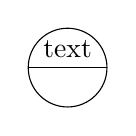
\begin{tikzpicture}
	\draw circle (0.5);
	\draw (-.5,0) to ["text"] (.5,0);
\end{tikzpicture}
\begin{tikzpicture}
	\draw[thin,dotted,step=0.5] (-3,-3) grid (3,3);
	\draw[->] (-3,0) -- (3,0);
	\draw[->] (0,-3) -- (0,3);
\end{tikzpicture}
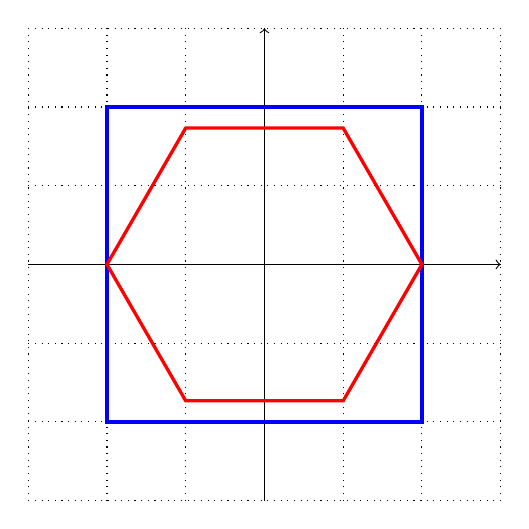
\begin{tikzpicture}
  \draw[thin,dotted] (-3,-3) grid (3,3);
  \draw[->] (-3,0) -- (3,0);
  \draw[->] (0,-3) -- (0,3);
  \draw[very thick, blue] (-2,-2) -- (-2,2)
    -- (2,2) -- (2,-2) -- cycle;
	\draw[very thick, red] (0:2) -- (60:2) -- (120:2)
	-- (180:2) --(240:2) -- (300:2) -- cycle;
\end{tikzpicture}
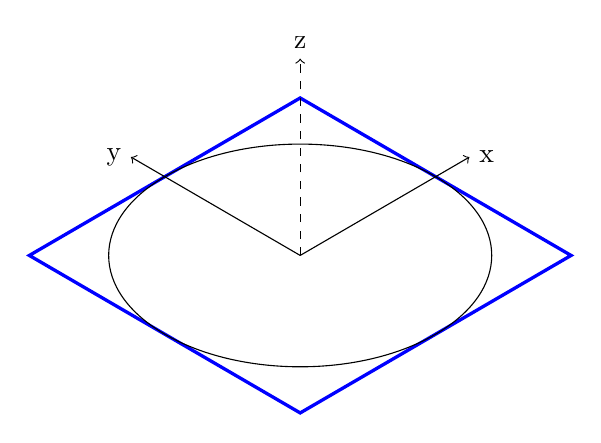
\begin{tikzpicture}[x={(0.86cm,0.5cm)},
  y={(-0.86cm,0.5cm)}, z={(0cm,1cm)}]
  \draw[very thick, blue] (-2,-2,0) -- (-2,2,0)
   -- (2,2,0) -- (2,-2,0) -- cycle;
  \draw[->] (0,0,0) -- (2.5, 0,  0) node [right] {x};
  \draw[->] (0,0,0) -- (0,  2.5, 0) node [left] {y};
  \draw[->,dashed] (0,0,0) -- (0,  0, 2.5) node [above] {z};
  \draw circle (2);
\end{tikzpicture}
\begin{tikzpicture}
	\draw[very thick, blue] (-3,-1) -- +(1,0)
  -- +(2,2) -- +(4,2) -- +(5,0) -- +(6,0);
	\draw[thin, dotted] (-3,-3) grid (3,3);
\end{tikzpicture}

\begin{tikzpicture}
	\draw[shading=ball, ball color=yellow] (0,0)
  circle [radius=2];
\draw[shading=ball, ball color=black] (-0.5,0.5,0)
  ellipse [x radius=0.2, y radius=0.4];
\draw[shading=ball, ball color=black] (0.5,0.5,0)
  ellipse [x radius=0.2, y radius=0.4];
\draw[very thick] (-1,-1) arc [start angle=185,
  end angle=355, x radius=1, y radius=0.5];
\end{tikzpicture}

\usetikzlibrary{datavisualization}
\begin{tikzpicture}
	\datavisualization [
		scientific axes=clean, 
		x axis = {
			attribute=batch_size, 
			ticks=many, length=\linewidth, label=batch size 
		},
		y axis = {
			attribute=time, 
			include value=0, 
			length=8cm, 
			label=time,
			ticks={tick unit=ns},
		},
		all axes={grid},
		visualize as scatter,
	] data [
		format=table, 
		read from file=data1.txt, 
		separator=\space,
		headline={batch_size time}
	];
\end{tikzpicture}


\begin{tikzpicture}
	\draw (4,2) node[draw, color=red, fill=yellow, text=blue] {TikZ};
\end{tikzpicture}



\begin{tikzpicture}
	\node[draw] at (4,2) {TikZ};
\end{tikzpicture}

\begin{tikzpicture}
	\node (r) at (0,1) [draw,rectangle] {rectangle};
	\node (c) at (1.5,0) [draw,circle] {circle};
	\node (e) at (3,1) [draw,ellipse] {ellipse};
	
	\draw[->] (r.east) -- (e.west);
	\draw[->] (r.south) -- (c.north west);
	\draw[->] (e.south west) -- (c.north east);
	%   n 
	% w   e
	%   s
\end{tikzpicture}

\begin{tikzpicture}
	\coordinate (begin) at (0,0);
	\coordinate (end) at (5,0);
	\draw (begin) -- (end);
\end{tikzpicture}

\begin{tikzpicture}
	\node[draw,shape=cloud] at (0,0) {text};
\end{tikzpicture}

\begin{tikzpicture}
	\node (student) [graduate, monitor, minimum size=2cm] at (1,1) {};
	\node at (student.45) [starburst, draw=red, fill=yellow, starburst point height=4mm, line width = .4pt, font = \ttfamily\scriptsize, inner sep=1.5pt] {error};
	\node at (student.130) [cloud callout, cloud puffs=13, aspect=3, anchor=pointer, shading=ball, ball color=gray, text=white, font=\bfseries] {My thesis\dots!};
\end{tikzpicture}

\begin{tikzpicture}
	\node [draw] (TikZ) {TikZ};
	\node [draw, right = 1mm of TikZ] {PDF};
\end{tikzpicture}

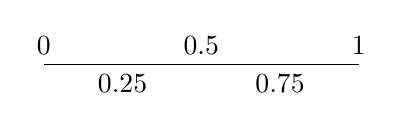
\begin{tikzpicture}
	\draw (0,0) --
		node [above, pos=0] {0}
		node [above, pos=0.5] {0.5}
		node [above, pos=1] {1}
		node [below, pos=0.25] {0.25}
		node [below, pos=0.75] {0.75}
	(4,0);
\end{tikzpicture}

\begin{tikzpicture}[every node/.style = {inner sep=0pt}]
  \node (E) {E};
  \node (p) [base right = 0pt of E] {p};
  \node (i) [base right = 0pt of p] {i};
  \node (c) [base right = 0pt of i] {c};
	\node (.) [base right = 0pt of c] {.};
\end{tikzpicture}


\begin{tikzpicture}
	\node[
		label = above:Graphics,
		label = left:Design,
		label = below:Typography,
		label = right:Coding,
		circle, shading=ball, ball color=blue!60, text=white]
		{TikZ};
\end{tikzpicture}

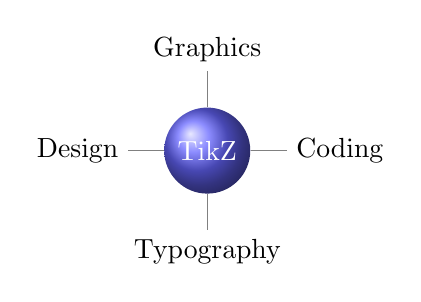
\begin{tikzpicture}
	\node[
		pin = above:Graphics,
		pin = left:Design,
		pin = below:Typography,
		pin = right:Coding,
		circle, shading=ball, ball color=blue!60, text=white]
		{TikZ};
\end{tikzpicture}

\end{document}
